\documentclass[11pt]{book}

\usepackage{amsfonts, amsmath, amssymb, color, mathrsfs, cite}
\usepackage{times}
\usepackage[usenames, dvipsnames ]{xcolor}  
\usepackage{arydshln}
\usepackage[ruled, vlined]{algorithm2e}
\usepackage{indentfirst}
\usepackage{hyperref}
\usepackage[section]{placeins}
\usepackage{graphicx}
\usepackage{listings}
\usepackage{float}
\usepackage{multirow}
\DeclareGraphicsExtensions{.pdf,.png,.jpg}

\setlength{\oddsidemargin}{1.5cm}
\setlength{\evensidemargin}{0cm}
\setlength{\topmargin}{1mm}
\setlength{\headheight}{1.36cm}
\setlength{\headsep}{1.00cm}
\setlength{\textheight}{19cm}
\setlength{\textwidth}{14.5cm}
\setlength{\marginparsep}{1mm}
\setlength{\marginparwidth}{3cm}
\setlength{\footskip}{2.36cm}

\newtheorem{thm}{Theorem}[section]
\newtheorem{lem}[thm]{Lemma}
\newtheorem{prop}{Proposition}[section]
\newtheorem{mydef}[thm]{Definition}
\newtheorem{cor}[thm]{Corollary}
\newtheorem{exam}[thm]{Example}
\newtheorem{rem}{Remark}

\newcommand{\ms}[1]{\mathscr{#1}}
\newcommand{\N}{\mathbb N}
\newcommand{\Q}{\mathbb Q}
\newcommand{\R}{\mathbb R}
\newcommand{\Z}{\mathbb Z}

\newcommand{\mynorm}[1]{\left\|#1\right\|}
\newcommand{\cone}[2]{K\!\left[#1;#2\right]}

\newenvironment{proof}{\paragraph{Proof:}}{\hfill$\square$}

%------------------------------------------------------------------------------
%                     THIS IS THE END OF THE PREAMBLE
%------------------------------------------------------------------------------


\begin{document}
\pagestyle{empty}

%------------------------------------------------------------------------------
%                     TITLE PAGE: name, degree,..
%------------------------------------------------------------------------------

\begin{center}

\vspace{1cm}

{\Huge Computing Optimum Covers of Functional Dependencies}

\vspace{75mm} 

{\Large Guangrui Wang}

\vspace{1ex}

Department of Computer Science

The University of Auckland

\vspace{5ex}

Supervisor: Professor Dr. Sebastian Link

\vspace*{60mm}

A thesis submitted in partial fulfilment of the requirements for the degree of Master of Professional Studies in Data Science, The University of Auckland, 2020.

\end{center}



%------------------------------------------------------------------------------
%                     FRONT MATTER:  abstract,..
%------------------------------------------------------------------------------

\chapter*{Abstract}       
\setcounter{page}{1}
\pagestyle{headings}

\addcontentsline{toc}{chapter}{Abstract}

Functional dependencies are important in relational databases as they formulate the constraints between different sets of attributes. There are different but equivalent ways to represent the same set of functional dependencies which are as known as covers. The performance of many data processing tasks such as data cleaning and query optimization deeply replies on how small the size of the cover is. In this article, we will talk about different types of "smallest covers" (optimum covers), how they can be calculated, how about the time consuming and how small they are.

\chapter*{Acknowledgement}       
\setcounter{page}{2}
\pagestyle{headings}

\addcontentsline{toc}{chapter}{Acknowledgement}

I would like to express my deepest appreciation to my supervisor Prof. Sebastian Link for his excellent guidance, suggestions and encouragement not only in this dissetation but also in other courses.

I would also like to extend my deepest gratitude to Dr. Ziheng Wei who helped a lot to review and guidance the implementation.

I am also grateful to my parents and my wife, for their unconditional love and support especially during this tough period against COVID-19.


%------------------------------------------------------------------------------
%                     CONTENTS
%------------------------------------------------------------------------------

\setcounter{secnumdepth}{3}
\setcounter{tocdepth}{3}
\tableofcontents

%: --------------------------------------------------------------
%:                  MAIN DOCUMENT SECTION
% --------------------------------------------------------------
	
\chapter{Introduction}

The term "relational database" was first introduced by Codd \cite{codd13f} from IBM in 1970. In the relational database model, the data are described in the form of relations. A relation can be represented as a table. Each row (except the header) indicates a relationship between a tuple of elements. Each column indicates a set of elements called an attribute.

\begin{table}[H]
	\centering
	
	\begin{tabular}{ c c c }
		A     & B     & C \\
		\hline
		$a_1$ & $b_1$ & $c_1$ \\ 
		$a_1$ & $b_2$ & $c_1$ \\ 
		$a_2$ & $b_1$ & $c_2$ \\
		$a_1$ & $b_2$ & $c_1$ \\
	\end{tabular}
	
	\caption{Some example of table}
	
	\label{example_table_1}
\end{table}

Functional dependencies (FDs) are used to constraint the relations. Let's say we have a relation $r$ and a functional dependency $f: X \rightarrow Y$, $r$ satisfies $f$ only if each set of tuples with equal $X$ values has equal $Y$ values \cite{maier1983theory}. Table \ref{example_table_1} shows some example table, it satisfies the functional dependency $f: AB \to C$, because when the values of A and B are determined, the value of C can also be uniquely determined.

\begin{table}[H]
	\centering
	
	\begin{tabular}{ c c c }
		A     & B     & C \\
		\hline
		$a_1$ & $b_1$ & $c_1$ \\
		\hdashline
		$a_1$ & $b_2$ & $c_1$ \\ 
		$a_1$ & $b_2$ & $c_1$ \\
		\hdashline		
		$a_2$ & $b_1$ & $c_2$ \\
	\end{tabular}
	
	\caption{Some example of table (sorted by A and B)}
\end{table}

A set of functional dependencies are usually called a cover. Given a cover, we may have different but equivalent representations. For example: $\{ A \to B, A \to C \}$ can be also represented as $\{ A \to BC \}$.

~\\
There are many scenarios where the size of functional dependencies is very important.
~\\

1) Data validation. Functional dependencies are used as integrity constraints to validate if the updates of a database are meaningful. If any update operation leads some violation of any functional dependency, then the update should be rejected, or at least some warning should be issued. Therefore, database management system must verify after every update whether the resulting database still satisfies all the functional dependencies that have been specified. To implement such a relational database system which supports functional dependencies, a simple idea could be to iterate each functional dependency $f$ and read related attributes of a relation after updating this relation. Obviously, the smaller the cover is, the less time it takes for the validation.

2) Data mining. For data analysis, datasets are often mined for the set of functional dependencies that hold on the given database.

3) Data normalization.
~\\

These use cases strongly motivate the question: What do the diffrent notions of covers achieve? To be more specific, the question can be divided into two parts: 1) How do the output sizes of the different cover algorithms compare against each other? 2) How do the times to compute the different covers compare against each other?

So far, the literature has not brought forward any experimental study focusing on these questions about different covers. Therefore, the main purpose of this article is trying to go deeper into the algorithms of different kinds of "minimum" covers and experimentally analysis the ratio between the time consumption of these algorithms and the reduction of the size of attributes. In Chapter 2., we will should some literature review of the notions of different covers. In Chapter 3., we will introduce the algorithms to compute different covers. In Chapter 4., we will show the experiment result and experimental comparision to quatify the trade-off.

\chapter{Literature Review}

In this chapter, we will introduce the formal definitions in relational database model including relations, functional dependencies, closures and covers. Then we'll talk about the notions of different kinds of covers from the previous literature.

\section{Relational Database Model}

\subsection{Relations}

The term relation was introduced by Codd \cite{codd13f} in 1970. He gaved a mathmatical sense to describe the Large Shared Data Banks as Relational Model of Data. 

\begin{mydef}
Given sets of attributes $S_1, S_2, \cdots, S_n$, a \textbf{relation} $r$ on these attribute sets is a set of n-tuples where the $i-th$ element $\in S_i$.
\end{mydef}

\subsection{Functional Dependencies}

The functional dependency can be seen as a special type of relationship between two sets of attributes under a given relation \cite{beeri1979computational}.

\begin{mydef}
Let's say $X$ and $Y$ are two sets of attributes chosen from a universe $U$ in a given database $D$, a \textbf{functional dependency} $f: X \rightarrow Y$ is such a constraint between $X$ and $Y$ in a relation $r$ of the database $D$. $r$ satisfies $f: X \rightarrow Y$ if and only if there are no such two entities $e_1$ and $e_2$ in $r$ where the $X$ values are equal but the $Y$ values are not equal.
\end{mydef}

\subsection{Closure}

\begin{mydef}
For a given set of functional dependencies $F$, the \textbf{closure} of $F$ is written $F^+$ which contains all the functional dependencies which can be inferenced by $F$. 
\end{mydef}

The closure can be calculated based on Armstrong's axioms.

\begin{thm}[reflexivity]
  $Y \subseteq X \Rightarrow X \to Y \in F^+$.
\end{thm}

\begin{thm}[projectivity]
  $X \rightarrow Y \in F^+ \land X \rightarrow Z \in F^+ \Rightarrow X \rightarrow YZ \in F^+$.
\end{thm}

\begin{thm}[transitivity]
  $X \rightarrow Y \in F^+ \land Y \rightarrow Z \in F^+ \Rightarrow X \rightarrow Z \in F^+$.
\end{thm}

\subsection{Covers}

\begin{mydef}
For a given set of functional dependencies $F$, we say $G$ is a \textbf{cover} of $F$ if and only if $G^+ = F^+$. And we also say two sets of functional dependencies $F$ and $G$ are \textbf{equivalent}, written $F \equiv G$, if $F^+ = G^+$.
\end{mydef}

\section{Different Types of Covers}

\subsection{Non-redundant Covers}

\begin{mydef}[Maier \cite{maier1980minimum}]
We say a cover $G$ is \textbf{non-redundant} if there is no such functional dependency $f \in G$ where $(G - \{f\}) \equiv G$.
\end{mydef}

\subsection{Canonical Covers}

\begin{mydef}[Paredaens \cite{paredaens1977functional}]
We say $G$ is a \textbf{canonical} cover if $G$ is \textbf{redundant} and for each functional dependency $f: X \rightarrow Y \in G$:
  \begin{itemize}
	\item the size of the left side $\lvert Y \rvert = 1$.
	\item there is no such $X^{'}$ where $X^{'} \subset X$ and $X^{'} \rightarrow Y \in G^{+}$.
  \end{itemize}
\end{mydef}

\subsection{Mini Covers}

\begin{mydef}[Peng \& Xiao \cite{peng2016optimal}]
We say $G$ is a \textbf{mini} cover if:
  \begin{itemize}
  	\item for each functional dependency $f: X \rightarrow Y \in G$, the size of the right side $\lvert Y \rvert = 1$.
  	\item with the first constraint, $G$ has the fewest number of functional dependencies.
  	\item with the first two constrains, $G$ has the fewest number of attributes (repetitively counted).
  \end{itemize}
\end{mydef}

\subsection{Minimum Covers}

\begin{mydef}[Maier \cite{maier1980minimum}]
We say $G$ is a \textbf{minimum} cover if there is no such $H$ where $H \equiv G$ and $\lvert H \rvert < \lvert G \rvert$.
\end{mydef}

\subsection{L-Minimum Covers}

\begin{mydef}[Maier \cite{maier1980minimum}]
We say $G$ is a \textbf{L-minimum} cover if:
  \begin{itemize}
  	\item $G$ is \textbf{minimum}.
  	\item for each functional dependency $f: X \rightarrow Y \in G$, there is no such $X^{'}$ where $X^{'} \subset X$ and $X^{'} \rightarrow Y \in F^{'}$.
  \end{itemize}
\end{mydef}

\subsection{LR-Minimum Covers}

\begin{mydef}[Maier \cite{maier1980minimum}]
We say $G$ is a \textbf{LR-minimum} cover if:
  \begin{itemize}
  	\item $G$ is \textbf{L-minimum}.
  	\item for each functional dependency $f: X \rightarrow Y \in G$, there is no such $Y^{'}$ where $(G - \{f\} + \{X \rightarrow Y^{'}\}) \equiv G$.
  \end{itemize}
\end{mydef}

\subsection{Optimal Covers}

\begin{mydef}[Maier \cite{maier1980minimum}]
We say $G$ is a \textbf{optimal} cover if there no such $H$ where $H \equiv G$ and $H$ has fewer number of attributes (repetitively counted).
\end{mydef}

\section{Relationships between Different Types of Covers}

Canonical, L-minimum, LR-minimum and optimal covers are the covers with only necessary attributes in the left sides. Canonical, LR-minimum and optimal covers are the covers with only necessary attributes in the right sides. Figure 2.1 shows the relationships between different definitions of covers. In the next section, we'll start to talk the algorithms to compute all these kinds of covers. Obviously, computing optimal cover should be most difficult task. And in the next section, we'll find that Non-redundant, Minimum, L-Minimum, LR-Minimum and Canonical covers can be calculated in non-exponential time. Mini and Optimal cover promblems are NP-Complete.

\begin{figure}
	\centering
	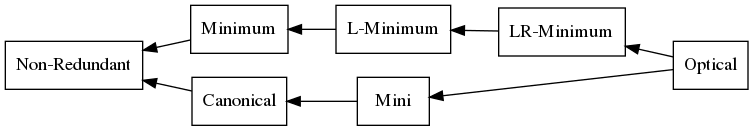
\includegraphics[width=\textwidth]{./diagrams/types-of-covers.png}
	\caption{Relationships between Different Types of Covers}
\end{figure}

\section{Related Works}

Maiver \cite{maier1980minimum} introduced the definitions of most different optimum covers (minimum, L-minimum, LR-minimum and optimal) mentioned in this paper. He also introduced an square-time algorithm to find the minimum cover. Beeri \& Bernstein \cite{beeri1979computational} introduced a linear-time algorithm to deal with the depend and membership problem. They also gave an procedure to remove redundant attributes from the left side of each functional dependency. Peng \& Xiao \cite{peng2016optimal} introduced a new concept called Mini Cover and indicated that the computation of Mini Cover can be equivalent to the computation of Minimum Boolean Expression. They also indicated that an Optimal Cover can be calculated via an OPTIMIZE algorithm from a Mini Cover.

\section{Summary}

In this chaper, we provided some literature review about the basic definitions in relational database model including relations, functional dependencies, closures and covers. And we also introduced the different notions of covers and the relationships between these covers. 

\chapter{Algorithms}

In this chapter, we'll first talk about some basic operations for computing covers including dependent set computation, membership determination, attributes equivalence determination and functional dependencies equivalence determination. Then, based on these basic operations, we'll introduce how to compute non-redundant cover, canonical cover, minimum cover, l-minimum cover and lr-minimum cover. After that, we'll move on the computation of mini cover. It can be transformed (Delobel-Casey Transform) as a minimum boolean expression problem. We'll talk about how to use Quine-McCluskey method to find candidate expressions and how to transform that problem again into a 0-1 integer programming model. Finally, based on the result of mini cover, we will show the algorithm to compute optimal cover.

\section{Dependent Set}

Before introducing the algorithms of different kinds of optimum covers, we first talk about how to find the dependent set from a given set of attributes $X$ under a given set of functional dependencies $F$. Algorithm 1. shows how to compute $\{ y \mid X \rightarrow \{ y \} \in F^{+} \}$ from Beeri \& Bernstein \cite{beeri1979computational}.

\begin{algorithm}

  \caption{depend(U, F, X)}
 
  \SetAlgoLined
  
  \For{$F_{i}: X \rightarrow Y \in F$} {
    count[i] = $\lvert X \rvert$;
    
    \For{$x \in X$} {
    	attrlist[x] = attrlist[x] $\cup\ \{ i \}$
    }
  }
  
  D = $\{ x \mid x \in X \}$;
  
  Q = a queue initialized with X;
  
  \While{Q is not empty} {
  	pop x from Q;
  	
  	\For{i $\in$ attrlist[x]} {
  		count[i] = count[i] - 1;
  		
  		\If{count[i] = 0} {
  			$f: X \rightarrow Y = F_i$
  			
  			\For{$y \in Y$}{
  				D = D $\cup\ \{ y \}$;
  				
  				push y into Q;
  			}
  		}
  	}
  }
  
  \Return{D};
\end{algorithm}

Where $U$ is the universe of attributes, $F$ is the given set of functional dependencies and $X$ is the given set of attributes. In this algorithm, we will first count the number of left side attributes in each functional dependency $count[i]$ and use a variable $attrlist[x]$ to indicate the indexes of functional dependencies where $x$ is in the left side. The following is a BFS-like approach.
If the left side attributes of a functional dependency $f$ can be fully determined from $X$, we will add it's right side attributes into the queue and iterate this process.

Since each functional dependency will be consumed only once, if we regard the length of each functional dependency as a constant, the time complexity should be $O(\lvert F \rvert)$.

\section{Membership Determination}

Based on the depend algorithm, we can easily determine if $X \rightarrow Y \in F^+$. Algorithm 2. shows the proccess how to determine if a given functional dependency $X \to Y$ belongs to the closure of a given functional dependnecy set $F$. Since the membership algorithm only takes extra $O(|Y|)$ time to check if $Y \subseteq depend(U, F, X)$, the time complexity of membership algorithm should be $O(|F|)$ as same as the depend algorithm.

\begin{algorithm}

  \caption{membership(U, F, X, Y)}

  \SetAlgoLined

  $Y^{'}$ = depend(U, F, X);
  
  \For{y $\in$ Y}{
  	\If{y $\not \in$ $Y^{'}$}{
  		\Return{false};
  	}
  }
  
  \Return{true};

\end{algorithm}

\section{Attributes Equivalence Determination}

Given two sets of attributes $X$ and $Y$, to determine if $X \equiv Y$ under a given set of functional dependency is equivalent to check if $X \rightarrow Y \in F^{+}$ and $Y \rightarrow X \in F^{+}$. Algorithm 3. shows this process. And the time complexity of determining attributes equivalence should be, as same as the time complexity of membership algorithm, $O(|F|)$.

\begin{algorithm}

  \caption{attr\_eq(U, F, X, Y)}
  
  \SetAlgoLined
    
  \eIf{membership(U, F, X, Y) $\land$ membership(U, F, Y, X)}{
  	\Return{true}
  }{
  	\Return{false}
  }
  
\end{algorithm}

\section{Functional Dependencies Equivalence Determination}

Given two sets of functional dependencies $F$ and $G$, to determine if $F \equiv G$, we can iterate each $f \in F$ to check if $f \in F^{+}$ and each $g \in G$ to check if $g \in G^{+}$. After these two iterations, we can determine if $F^{+} \subseteq G^{+}$ and $G^{+} \subseteq F^{+}$, which is equivalent to $F^{+} = G^{+}$. Algorithm 3. shows this process. Since we need to run $|F|$ times membership algorithm among $G$ and $|G|$ times membership algorithm among $F$, the overall time complexity should be $O(|F| \times |G|)$.

\begin{algorithm}

  \caption{fd\_eq(U, F, G)}
  
  \SetAlgoLined
  
  \For{$f: X \rightarrow Y \in F$}{
  	\If{$\lnot$ membership(U, G, X, Y)}{
  		\Return{False};
  	}
  }
  
  \For{$g: X \rightarrow Y \in G$}{
  	\If{$\lnot$ membership(U, F, X, Y)}{
  		\Return{False};
  	}
  }

  \Return{true};
  
\end{algorithm}

\section{Non-Redundant Cover}

Given a set of functional dependencies $F$, to compute a non-redundant cover $G$ where $G \equiv F$ and for each $H \subset G$, $H \not \equiv F$, we can iterate each functional dependency $f \in F$, if $f \in (F - \{ f \})^{+}$, then $f$ should be removed from the result $G$. Algorithm 5. shows this process. Basically, it takes membership algorithm for $|F|$ times; so the time complexity should be $O(|F|^2)$.

\begin{algorithm}

  \caption{non\_redundant(U, F)}
  
  \SetAlgoLined
  
  G = $\varnothing$;
  
  \For{$f: X \rightarrow Y \in F$} {
    $X^{'}$ = $X$;
    
    \If{$\lnot$ membership(U, $F - \{f\}$, X, Y)} {
    	G = $G \cup \{ f \}$;
    }
  }
  
  \Return{G};

\end{algorithm}

\section{Canonical Cover}

Algorithms 6. shows how we compute a canonical cover. To compute a canonical cover of a given set of functional dependencies $F$, first we should split the right side of each funtional dependency to make sure the size of right side is single and convert it to a non-redundant cover. Then we can use the algorithm introduced by Beeri \& Bernstein \cite{beeri1979computational} to remove left side extraneous attributes. Every time we can apply a linear-time membership algorithm to check if $(X - {B}) \to A \in F^{+}$. If so, we replace $X$ with $X - {B}$. Since we may run membership algorithm at most $|F|$ times. The time complexity of canonical algorithm is $O(|F|^2)$.

\begin{algorithm}

  \caption{canonical(U, F)}
  
  \SetAlgoLined
  
  G = $\varnothing$;

  \For{$f: X \rightarrow Y \in F$} {
  	\For{$y \in Y$}{
  		G = $G \cup \{ X \rightarrow \{ y \}\}$;
  	}
  }
  
  G = non\_redundant(G);
  
  H = $\varnothing$;
  
  \For{$g: X \rightarrow Y \in G$} {
    $X^{'}$ = X;
     	
  	\For{$x \in X$}{
  		
  		\If{membership$(U, F, X^{'} - \{x\}, Y)$}{
  		  $X^{'}$ = $X^{'} - \{ x \}$;
  		}
  		
  		H = $H \cup \{ X^{'} \rightarrow Y \}$;
  	}
  }
  
  \Return{H};
  
\end{algorithm}

\section{Minimum Cover}

In Maier 1980 \cite{maier1980minimum}, the author introduced an $O(|F|^2)$ algorithm to compute the minimum cover. Algorithm 7. shows the process how we compute a minimum cover under a given universe $U$ and a functional dependency set $F$. The main idea is that we first convert the functional dependency set $F$ to a non-redudant cover $G$. And then, we iterate all pairs of functional dependency $X_i \rightarrow Y_i \in G$ and $X_j \rightarrow Y_j \in G$, if we find such pair of functional dependencies where $X_i \leftrightarrow X_j$ and $X_i \rightarrow Y_j \in G^{+}$, we can replace the two functional dependencies with a new one: $X_j \rightarrow Y_iY_j$. Since we may iterate all pairs of functional dependnecies, the time complexity of minimum cover algorithm is $O(|F|^2)$.

\begin{algorithm}
  \caption{minimum(U, F)}
  
  \SetAlgoLined
  
  G = non\_redundant(F);
  
  \For{$X \rightarrow Y \in G$} {
  	D[X] = depend(U, G, X);
  }
  
  \For{$X_i \rightarrow Y_i \in G$} {
  	\For{$X_j \rightarrow Y_j \in G$} {
  	  M[i][j] = $X_j \subseteq X_i$;  	
  	}
  }
  
  \For{$X_i \rightarrow Y_i \in G$} {
    $D^{'}$ = depend(U, G, $X_i$);
    
    \For{$X_j \rightarrow Y_i \in G$} {
      \If{$i \neq j \land M[i][j] \land M[j][i] \land X_j \subseteq D^{'}$} {
      	G = $G - {X_i \rightarrow Y_i}$;
      	
      	G = $G - {X_j \rightarrow Y_j}$;

      	G = $G \cup {X_j \rightarrow Y_iY_j}$;
      }
    }    
  }
\end{algorithm}

\section{L-Minimum Cover}

The computation of L-minimum cover is based on the computation of minimum cover. By using the same algorithm \cite{beeri1979computational} mentioned in \textbf{3.6 canonical} to remove extranous left side attributes, we can convert a minimum cover to a L-minimum cover. Algorithm 8. shows the process of L-minimum cover algorithm. It first converts the given functional dependency $F$ to a minimum cover $G$. And then every time it applies a linear-time membership algorithm to check if $(X - B) \rightarrow A \in F^{+}$. If so, replace $X$ with $X - B$. The time complexity of computing L-minimum cover should be as same as the time complexity of minimum cover algorithm, $O(|F|^2)$.

\begin{algorithm}
 
  \caption{l\_minimum(U, F)}
  
  \SetAlgoLined
  
  G = minimum(U, F);
  
  H = $\varnothing$;
  
  \For{$g: X \rightarrow Y \in G$} {
    $X^{'}$ = X;
     	
  	\For{$x \in X$}{
  		
  		\If{membership$(U, F, X^{'} - \{x\}, Y)$}{
  		  $X^{'}$ = $X^{'} - \{ x \}$;
  		}
  		
  		H = $H \cup \{ X^{'} \rightarrow Y \}$;
  	}
  }
  
  \Return{H};

\end{algorithm}

\section{LR-Minimum Cover}

The computation of LR-minimum cover is based on the computation of L-minimum cover. 
Algorithm 9. shows the process of computing LR-minimum cover. For a functional dependency $f: X \rightarrow Y \in F$ if there is $Y^{'} \subset Y$ where $f \in (F - \{f\} + \{ X \rightarrow Y^{'} \})^{+}$, then we should replace $Y$ with $Y^{'}$. The time complexity of this algorithm is also $O(|F|^2)$, as same as the previous two algorithms.

\begin{algorithm}

  \caption{lr\_minimum(U, F)}
  
  \SetAlgoLined
  
  G = lminimum(U, F);
  
  H = $\varnothing$;
  
  \For{$f: X \rightarrow Y \in G$} {
  
    $Y^{'}$ = $Y$;
    
  	\For{$y \in Y$}{
  	  $G^{'}$ = $G - \{ f \} + \{ X \rightarrow (Y^{'} - \{ y \}) \}$;
  	
  	  \If{membership($U, G^{'}, X, Y$)} {
  	    $Y^{'}$ = $Y^{'} - \{ y \}$; 
  	  }
  	}
  	
  	$H$ = $H \cup \{ X \rightarrow Y^{'} \}$;
  }
  
  \Return{H};

\end{algorithm}

\section{Mini Cover}

\subsection{Delobel-Casey Transform}

The concept of mini cover was introduced by Peng \& Xiao \cite{peng2016optimal}. And the authors introduced an idea that the computation of mini cover is equivalent to the minimum boolean expression problem.

By using the first Delobel-Casey tranform \cite{delobel1973decomposition}, a functional dependency $f: X_1 X_2 \cdots X_m \rightarrow Y_1 Y_2 \cdots Y_n$ can be transformed to a boolean expression $X_1 X_2 \cdots X_m \overline{Y_1} + \cdots + X_1 X_2 \cdots X_m \overline{Y_m}$. And a set of functional dependencies $F$ can be transformed to the boolean sum of the transforms of each functional dependency.

For example, the Delobel-Casey transform of $F_1: \{ AB \rightarrow C, AB \rightarrow D, C \rightarrow D \}$ should be $b_1: AB\overline{C} + AB\overline{D} + C\overline{D}$. Since $AB\overline{D} = ABC\overline{D} + AB\overline{C}\overline{D}$, $ABC\overline{D}$ can be covered by $C\overline{D}$ and $AB\overline{C}\overline{D}$ can be covered by $AB\overline{C}$. $AB\overline{D}$ is redundant in the boolean expression $b_1$. So the minimum boolean expression of $b_1$ should be $b_2 = AB\overline{C} + C\overline{D}$. And $b_2$ can be transformed reversely to $F_2: \{ AB \rightarrow C, AB \rightarrow D, C \rightarrow D \}$.

Minimum boolean expression problem aims to find the equivalent boolean expression with fewest number of symbols (repeated).

\subsection{Quine-McCluskey Method}

By converting a given set of functional dependencies $F$, we get an equivalent minimum boolean expression problem for computing mini cover. Quine-McCluskey method \cite{mccluskey1956minimization} is a traditional algorithm to deal with minimum boolean expression problem.

Let's take the example in the previous section. We get a boolean expression $b_1: AB\overline{C} + AB\overline{D} + C\overline{D}$ from the given functional dependency set $F_1: \{ AB \rightarrow C, AB \rightarrow D, C \rightarrow D \}$. First, we write the function as a table iterating all the possible values of attributes and the related desired output. Table 3.1 shows the table of the function $F_1$. Then, we'll try to iterate paris of the terms and try to combine the pairs of terms $m_i$ and $m_j$ where $m_i$ and $m_j$ has only one different column (0 or 1). Table 3.2 shows how we combine the pairs of terms and find prime implicants. Then, we will try to find the combination of implicants (with minimum total number of symbols) to cover all the original terms in Table 3.1. As shown in the Table 3.3, the best solution should be choosing $m(2, 6, 10, 14)$ and $m(12, 13)$. So the equivalent minimum boolean expression should be $b_2 = AB\overline{C} + C\overline{D}$. 

\begin{table}
	\centering
	
	\begin{tabular}{ |c|c|c|c|c|c| }
		\hline
		  & A & B & C & D & F \\
		\hline
		 0 & 0 & 0 & 0 & 0 & 0 \\
		 1 & 0 & 0 & 0 & 1 & 0 \\
		 2 & 0 & 0 & 1 & 0 & 1 \\
		 3 & 0 & 0 & 1 & 1 & 0 \\
		 4 & 0 & 1 & 0 & 0 & 0 \\
		 5 & 0 & 1 & 0 & 1 & 0 \\
		 6 & 0 & 1 & 1 & 0 & 1 \\
		 7 & 0 & 1 & 1 & 1 & 0 \\
		 8 & 1 & 0 & 0 & 0 & 0 \\
		 9 & 1 & 0 & 0 & 1 & 0 \\
		10 & 1 & 0 & 1 & 0 & 1 \\
		11 & 1 & 0 & 1 & 1 & 0 \\
		12 & 1 & 1 & 0 & 0 & 1 \\
		13 & 1 & 1 & 0 & 1 & 1 \\
		14 & 1 & 1 & 1 & 0 & 1 \\
		15 & 1 & 1 & 1 & 1 & 0 \\			
		\hline
	\end{tabular}

	\caption{The table of function $F_1$}
\end{table}

\begin{table}
	\centering
	
	\begin{tabular}{c|c|c|c}
		\hline
		Number of 1s & Original terms & Size 2 implicants & Size 4 implicants \\
		\hline
		1 &  m(2) : 0010 &   m(2, 6) : 0x10 & m(2, 6, 10, 14) : xx10 \\
		  &              &  m(2, 10) : x010 \\ 
		\hline
		2 &  m(6) : 0110 &  m(6, 14) : x110 \\
		  & m(10) : 1010 & m(10, 14) : 1x10 \\
		  & m(12) : 1100 & m(12, 13) : 110x \\
		  &              & m(12, 14) : 11x0 \\
		\hline
		3 & m(13) : 1101 \\
		  & m(14) : 1110 \\
		\hline
	\end{tabular}
	
	\caption{Find prime implicants}
\end{table}

\begin{table}
	\centering
	
	\begin{tabular}{c|c|c|c|c|c|c}
		\hline
		& 2 & 6 & 10 & 12 & 13 & 14 \\
		\hline
		m(2,6,10,14) & $\surd$ & $\surd$ & $\surd$ &         &         & $\surd$ \\
		m(12, 13)    &         &         &         & $\surd$ & $\surd$ &         \\
		m(12, 14)    &         &         &         & $\surd$ &         & $\surd$ \\
		\hline
	\end{tabular}
	
	\caption{Prime implicant chart}
\end{table}

\subsection{Integer Programming Problem}

The remaining problem in the previous section is how we can find the best combination of implicants with minimum number of symbols. One simple solution could be using a $O(2^m)$ searching approach (where $m$ is the number of prime implicants generated after Quine-McCluskey method). But here, we have another solution. This problem can be easily converted to a equivalent 01-Integer programming problem.

Let's say we have a matrix $M$ where $C_{i, j} \in {0, 1}$ indicates whether the $i-th$ prime implicant contains the $j-th$ original term. And $S_{i} \in Z^{+}$ indicates the number of symbols contained in the $i-th$ prime implicant. $Z_i$ indicates whether we use the $i-th$ prime implicant in the result or not. Then we have:

\begin{align}
	Z_i \in {0, 1} & \\
	\forall j, \sum_{i} Z_i * M_{i, j} \geq 0 \\
	\min_{Z} \sum_{i} Z_i * S_{i}		 
\end{align}

So we converted the last step of Quine-McCluskey method into a pure 0-1 integer programming problem. Although 0-1 integer programming problem is still NP-Complete, it is helpful to make it descriptive. And in real engineering, we may use some common integer programming solver library to have better performance. Since the first step, we may need to iterate exponential-level number of terms and the final integer programming solving may also take exponential time. The overall time complexity of computing mini cover is still exponential level.

\section{Optimal Cover}

Now, let's go into the hardest problem, optimal cover. As introduced in Peng \& Xiao \cite{peng2016optimal}, with a given mini cover, we can get a equivalent optimal cover by applying the same MINIMIZE approach used in section 3.7. So here we can use a very similar approach to compute optimal cover. Algorithm 10. shows the process how we compute a optimal cover from a given functional dependency set $F$ under a given universe $U$. Since the step computing mini cover is NP-Complete,
the overall time complexity of computing optimal cover is still NP-Complelte.

\begin{algorithm}
  \caption{optimal(U, F)}
  
  \SetAlgoLined
  
  G = mini(U, F);
  
  \For{$X \rightarrow Y \in G$} {
  	D[X] = depend(U, G, X);
  }
  
  \For{$X_i \rightarrow Y_i \in G$} {
  	\For{$X_j \rightarrow Y_j \in G$} {
  	  M[i][j] = $X_j \subseteq X_i$;  	
  	}
  }
  
  \For{$X_i \rightarrow Y_i \in G$} {
    $D^{'}$ = depend(U, G, $X_i$);
    
    \For{$X_j \rightarrow Y_i \in G$} {
      \If{$i \neq j \land M[i][j] \land M[j][i] \land X_j \subseteq D^{'}$} {
      	G = $G - {X_i \rightarrow Y_i}$;
      	
      	G = $G - {X_j \rightarrow Y_j}$;

      	G = $G \cup {X_j \rightarrow Y_iY_j}$;
      }
    }    
  }
\end{algorithm}

\section{Implementation}

We implemented all the algorithms mentioned in the this chapter using C++ (around 1700 lines of code) and the project is fully open sourced on Github \cite{githubfdc}. We used the Standard Template Library (STL) \cite{plauger2000c++} to construct basic data structures, Lohmann's JSON library \cite{nlohmann_json} to deal with the format of our datasets and GNU Linear Programming Kit (GLPK) \cite{makhorin2008glpk} to solve some integer programming problem for computing optimal covers. We also used Google's GTest \cite{barca2016gtest} during development process to set up enough test cases validating the correctness of the implementions.

\section{Summary}

So in this chapter, we introduced some basic algorithms to find dependent set, validate membership determination, attributes equivalence and functional dependencies equivalence. Based on these basic approaches, we introduced how to compute non-redundant cover, canonical cover, minimum cover, l-minimum cover and lr-minimum cover. And then we talked about the computation of mini cover. It can be converted to a equivalent minimum boolean expression problem using Delobel-Casey transform. To solve the minimum boolean expression problem, we introduced Quine-McCluskey method and 0-1 integer programming model. Finally, based on the computation of mini cover, we introduced the optimal cover algorithm.

\chapter{Experiments}

In this chapter, we'll show some experiment results based on our c++ implementation and 11 datasets (mostly from realworld).



\section{Experiment Setup}

To evaluate the performance of different optimum cover algorithms, we used 12 different datasets for testing. Table 4.1 shows the characteristics of the 12 different databsets. Fd\_reduced is the only synthetic dataset. Other datasets are from realworld, obtained from the UCI Machine Learning Repository \cite{asuncion2007uci}

\begin{table}

	\centering
	
	\begin{tabular}{ |c|c|c| }
		\hline
		Dataset & Attributes & FDs \\
		\hline
		abalone        & 9 & 54 \\
		letter         & 17 & 61 \\
		adult          & 15 & 68 \\
		lineitem       & 16 & 901  \\ 
		china\_weather & 18 & 2955 \\ 
		fd\_reduced    & 30 & 3573 \\
		hepatitis      & 20 & 5372 \\
		uniprot        & 30 & 5794 \\
		horse          & 28 & 86583 \\
		diabetic       & 30 & 97341 \\
		plista         & 63 & 111360 \\
		flight         & 109 & 268262 \\
		\hline
	\end{tabular}

	\caption{Summary Characteristics of Various Datasets}
	
\end{table}

And our experiment runs on the same Linux laptop (Ubuntu 18.04.1, x86\_64, Intel i7-7700 HQ, 2.80GHz). 

\section{Experiment for Non-exponential Algorithms}

In this section, we only test the non-exponential time complexity algorithms (non-redundant, cannonical, minimum, L-minimum and LR-minimum algorithms). For each dataset, we first sorted the functional dependencies by ascending order. Then we tested 100 times for the algorithms. For each time, we only used the first $k$ ($k$ is from 1 to 100) percentage of the functional dependencies as the input. And we recorded the time consumption and the number of attributes in the result cover for each algorithm.

The line charts below show the experiment result for this section. Each pair of line charts indicates the result from one dataset. The both x-axises indicate the percentage of dataset we used as the input. For the left diagrams, the y-axis indicates the number of attributes (repetitvely counted) in the result cover for each algorithm. For the right diagrams, the y-axis indicates the time consumption for each algorithm.

Table 4.2-4.3 shows the time consumption and the result cover size for each algorithm and each dataset when using full functional dependencies as the input.

\begin{figure}
	\centering
	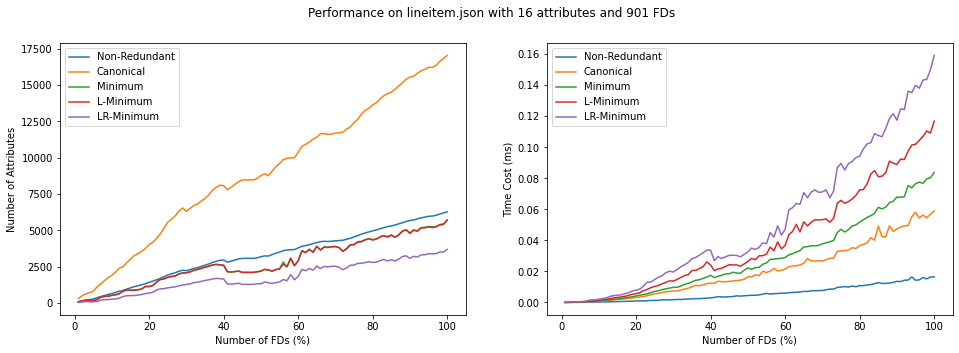
\includegraphics[width=\textwidth]{./diagrams/lab1/lineitem.png}
	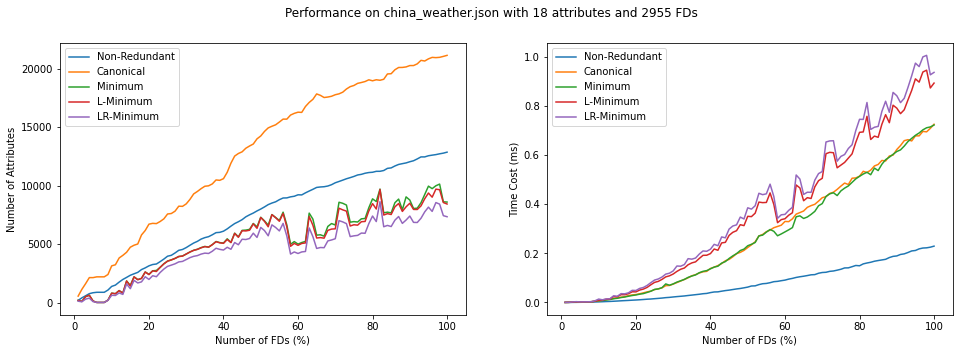
\includegraphics[width=\textwidth]{./diagrams/lab1/china_weather.png}
	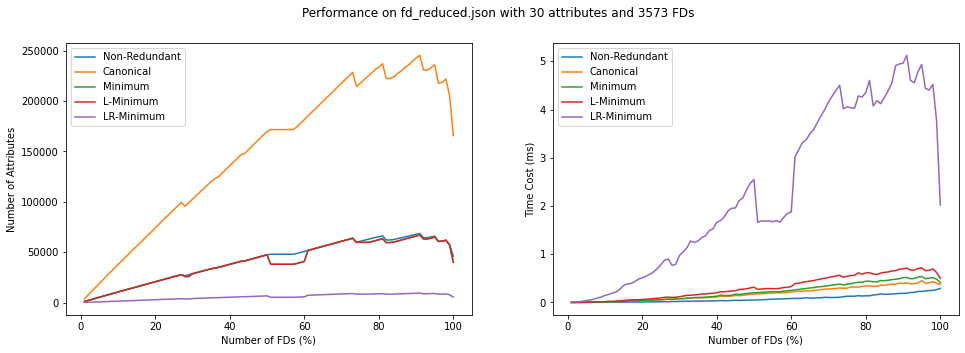
\includegraphics[width=\textwidth]{./diagrams/lab1/fd_reduced.png}
	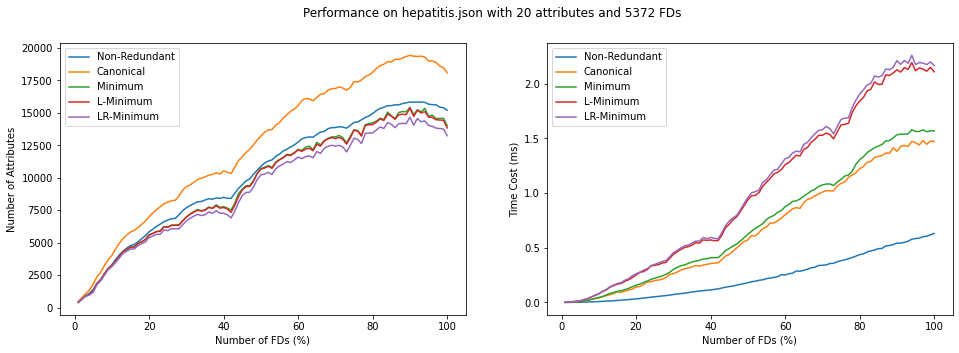
\includegraphics[width=\textwidth]{./diagrams/lab1/hepatitis.png}
\end{figure}

\begin{figure}
	\centering
	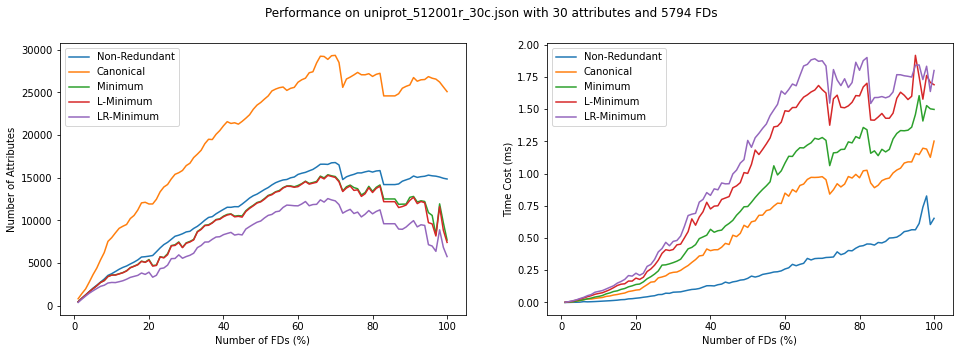
\includegraphics[width=\textwidth]{./diagrams/lab1/uniprot.png}
	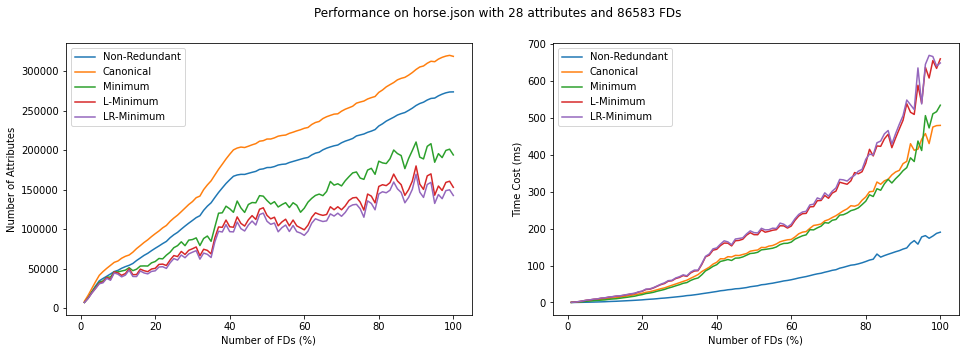
\includegraphics[width=\textwidth]{./diagrams/lab1/horse.png}
	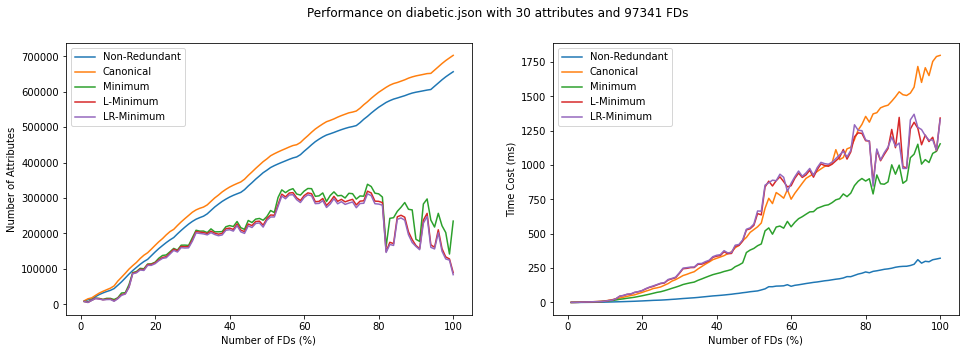
\includegraphics[width=\textwidth]{./diagrams/lab1/diabetic.png}
	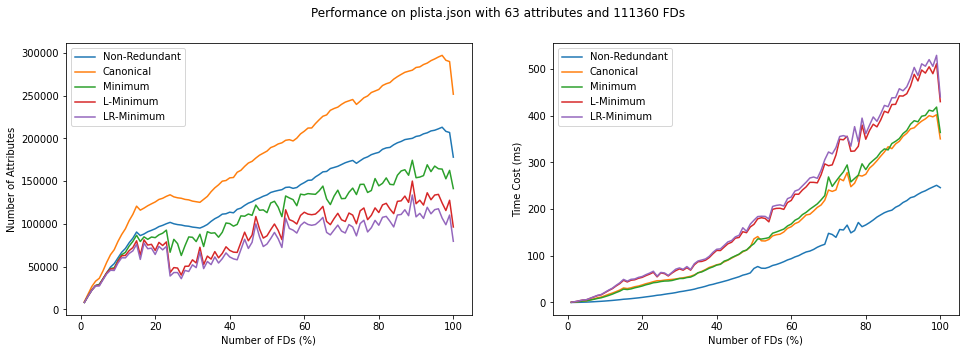
\includegraphics[width=\textwidth]{./diagrams/lab1/plista.png}
\end{figure}

\begin{figure}
	\centering
	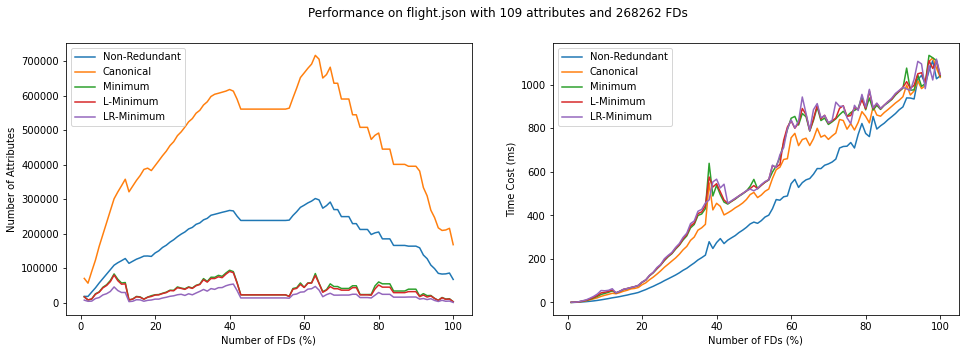
\includegraphics[width=\textwidth]{./diagrams/lab1/flight.png}
\end{figure}

\begin{table}[H]

	\centering
	
\begin{tabular}{|c|c|c|c|}

    \hline
    Dataset & Algorithm & Time consumption (sec) & Cover size \\
    
    \hline
    \multirow{5}{*}{lineitem}
    	& Non-Redundant & 0.017 & 6284  \\
    	& Canonical     & 0.059 & 17049 \\
    	& Minimum       & 0.084 & 5737  \\
    	& L-Minimum     & 0.117 & 5709  \\
    	& LR-Minimum    & 0.159 & 3700  \\
    
    \hline
    \multirow{5}{*}{china\_weather}
    	& Non-Redundant & 0.229 & 12868 \\
    	& Canonical     & 0.726 & 21142 \\
    	& Minimum       & 0.722 & 8602  \\
    	& L-Minimum     & 0.893 & 8435  \\
    	& LR-Minimum    & 0.937 & 7349  \\    	

    \hline
    \multirow{5}{*}{fd\_reduced}
    	& Non-Redundant & 0.290 & 46042  \\
    	& Canonical     & 0.376 & 165594 \\
    	& Minimum       & 0.414 & 39917  \\
    	& L-Minimum     & 0.499 & 39917  \\
    	& LR-Minimum    & 0.219 & 5340   \\

    \hline
    \multirow{5}{*}{hepatitis}
    	& Non-Redundant & 0.630 & 15206  \\
    	& Canonical     & 1.470 & 18093  \\
    	& Minimum       & 1.567 & 14008  \\
    	& L-Minimum     & 2.108 & 13844  \\
    	& LR-Minimum    & 2.165 & 13239  \\

    \hline
    \multirow{5}{*}{uniprot}
    	& Non-Redundant & 0.653 & 14848  \\
    	& Canonical     & 1.252 & 25080  \\
    	& Minimum       & 1.498 & 7701   \\
    	& L-Minimum     & 1.690 & 7424   \\
    	& LR-Minimum    & 1.800 & 5764   \\

    \hline
    \multirow{5}{*}{horse}
    	& Non-Redundant & 190.415 & 273647  \\
    	& Canonical     & 479.815 & 318631  \\
    	& Minimum       & 534.537 & 193863   \\
    	& L-Minimum     & 660.160 & 152868   \\
    	& LR-Minimum    & 648.983 & 142482   \\	
    	
    \hline
    
\end{tabular}

	\caption{Time Consumption and Cover Size of Non-exponential Algorithms}
	
\end{table}

\begin{table}[H]

	\centering
	
\begin{tabular}{|c|c|c|c|}

    \hline
    Dataset & Algorithm & Time consumption (sec) & Cover size \\
    
    \hline
    \multirow{5}{*}{diabetic}
    	& Non-Redundant & 321.835  & 656457 \\
    	& Canonical     & 1798.100 & 702696 \\
    	& Minimum       & 1154.360 & 234914 \\
    	& L-Minimum     & 1341.980 & 89483  \\
    	& LR-Minimum    & 1331.660 & 83712  \\	

    \hline
    \multirow{5}{*}{plista}
    	& Non-Redundant & 245.758 & 178077 \\
    	& Canonical     & 350.197 & 251700 \\
    	& Minimum       & 363.911 & 141314 \\
    	& L-Minimum     & 429.861 & 96389  \\
    	& LR-Minimum    & 439.981 & 79671  \\
    	
    \hline
    \multirow{5}{*}{flight}
    	& Non-Redundant & 1040.280 & 67090  \\
    	& Canonical     & 1033.250 & 167867 \\
    	& Minimum       & 1038.800 & 2563   \\
    	& L-Minimum     & 1042.440 & 2541   \\
    	& LR-Minimum    & 1047.610 & 436    \\
    	
    \hline
    
\end{tabular}

	\caption{Time Consumption and Cover Size of Non-exponential Algorithms}
	
\end{table}

\section{Experiment for All Algorithms}

Since the computation of mini covers and optimal covers is exponential time complexity, we cannot run the mini cover algorithm and the optimal cover algorithm for big datasets in a limited time. So in this section, we tested all the algorithms on three data sets where the size is limited.

And the approach is as same as the previous one. For each dataset, we first sorted the functional dependencies by ascending order. Then we repeated the test for 100 times. For each time, we only used the first $k$ ($k$ from 1 to 100) percentage of functional dependencies as the input and recorded the time consumption and the number of attributes (repetitively counted) in the result cover for each algorithm.

The digrams shown below indicate the experiment result for this section. As same as the previous diagrams, both x-axises represent the percentage of functional dependencies we used for one specific test. The y-axis in left diagrams represents the number of attributes in the result cover. And the y-axis in the right diagrams represents the time consumption.

Table 4.4 shows the time consumption and the result cover size for each algorithm and each dataset when using full data set as the input.

\begin{figure}
	\centering
	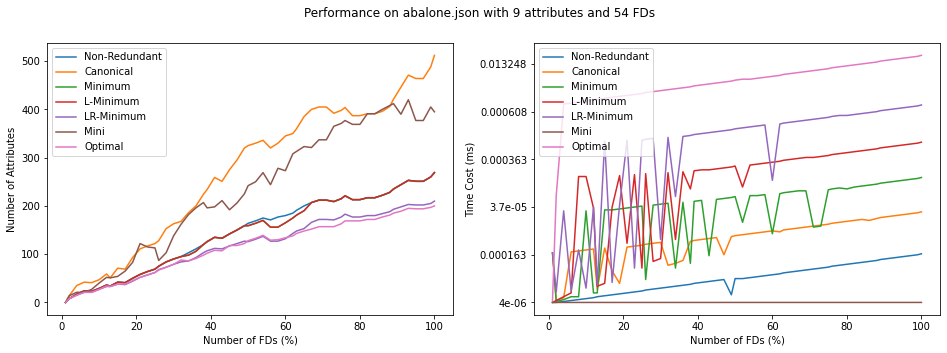
\includegraphics[width=\textwidth]{./diagrams/lab2/abalone.png}
	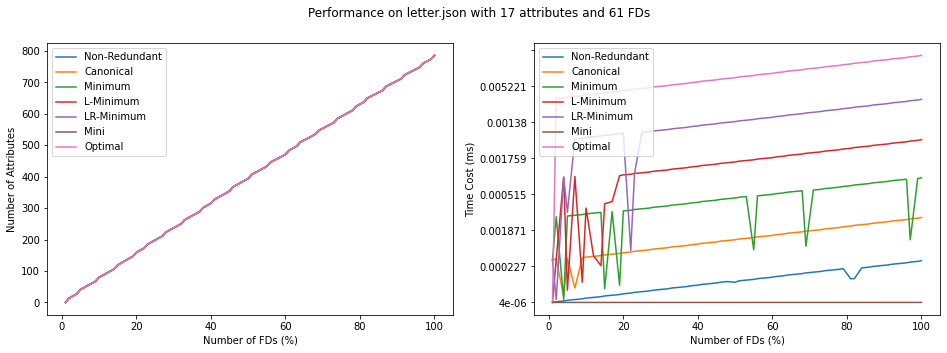
\includegraphics[width=\textwidth]{./diagrams/lab2/letter.png}
	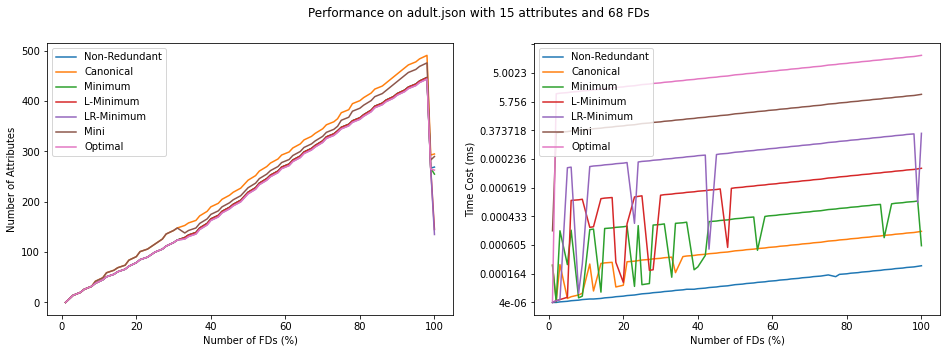
\includegraphics[width=\textwidth]{./diagrams/lab2/adult.png}
\end{figure}

\begin{table}[H]

	\centering
	
\begin{tabular}{|c|c|c|c|}

    \hline
    Dataset & Algorithm & Time consumption (sec) & Cover size \\
    
    \hline
    \multirow{5}{*}{abalone}
    	& Non-Redundant & 0.001 & 269 \\
    	& Canonical     & 0.001 & 512 \\
    	& Minimum       & 0.001 & 269 \\
    	& L-Minimum     & 0.001 & 269 \\
    	& LR-Minimum    & 0.001 & 210 \\	
    	& Mini          & 0.016 & 395 \\	
    	& Optimal       & 0.016 & 200 \\

    \hline
    \multirow{5}{*}{letter}
    	& Non-Redundant & 0.001 & 786 \\
    	& Canonical     & 0.003 & 786 \\
    	& Minimum       & 0.001 & 786 \\
    	& L-Minimum     & 0.004 & 786 \\
    	& LR-Minimum    & 0.004 & 786 \\	
    	& Mini          & 0.022 & 786 \\	
    	& Optimal       & 0.023 & 786 \\

    \hline
    \multirow{5}{*}{adult}
    	& Non-Redundant & 0.001  & 269 \\
    	& Canonical     & 0.001  & 295 \\
    	& Minimum       & 0.001  & 255 \\
    	& L-Minimum     & 0.001  & 145 \\
    	& LR-Minimum    & 0.001  & 135 \\	
    	& Mini          & 40.560 & 290 \\	
    	& Optimal       & 40.115 & 130 \\
	
    \hline
    
\end{tabular}

	\caption{Time Consumption and Cover Size of All Algorithms}
	
\end{table}

\section{Trade-off between Cover Size and Time Consumption}

To better understand the experiment result, for each dataset and each pairs of algorithms we compute the observed trade-off between the result cover size and the time consumption. Table 4.5 and Table 4.6 illustrate the time consumption ratio between each pairs of algorithms for each dataset. Table 4.7 and Table 4.8 indicate the result cover size ratio between each pairs of algorithms for each dataset.

And Table 4.9 and Table 4.10 show the overall ratio between each pairs of algorithsm for each dataset. In terms of over ratio, for a pair of algorithms $A$ and $B$, the ratio is calculated by:

$$
\frac
	{\text{B's cover size} \times \text{B's time consumption}}
	{\text{A's cover size} \times \text{A's time consumption}}
$$

\begin{table}

	\centering
	
\begin{tabular}{|c|c|c|c|c|c|c|c|c|}

    \hline
    Dataset &
    	Algorithm &
    	NR &
    	C &
    	Min &
    	L-Min &
    	LR-Min \\
    	    
    \hline
    \multirow{5}{*}{lineitem}
         & NR & 1.000 & 3.471 & 4.941 & 6.882 & 9.353 \\                                                                                                                                                             
         & Can & 0.288 & 1.000 & 1.424 & 1.983 & 2.695 \\                                                                                                                                                            
         & Min & 0.202 & 0.702 & 1.000 & 1.393 & 1.893 \\                                                                                                                                                            
         & L-Min & 0.145 & 0.504 & 0.718 & 1.000 & 1.359 \\                                                                                                                                                          
         & LR-Min & 0.107 & 0.371 & 0.528 & 0.736 & 1.000 \\ 	

    \hline
    \multirow{5}{*}{china\_weather}
         & NR & 1.000 & 3.170 & 3.153 & 3.900 & 4.092 \\                                                                                                                                                             
         & Can & 0.315 & 1.000 & 0.994 & 1.230 & 1.291 \\                                                                                                                                                            
         & Min & 0.317 & 1.006 & 1.000 & 1.237 & 1.298 \\                                                                                                                                                            
         & L-Min & 0.256 & 0.813 & 0.809 & 1.000 & 1.049 \\                                                                                                                                                          
         & LR-Min & 0.244 & 0.775 & 0.771 & 0.953 & 1.000 \\
         
    \hline
    \multirow{5}{*}{fd\_reduced}
         & NR & 1.000 & 1.297 & 1.428 & 1.721 & 0.755 \\                                                                                                                                                             
         & Can & 0.771 & 1.000 & 1.101 & 1.327 & 0.582 \\                                                                                                                                                            
         & Min & 0.700 & 0.908 & 1.000 & 1.205 & 0.529 \\                                                                                                                                                            
         & L-Min & 0.581 & 0.754 & 0.830 & 1.000 & 0.439 \\                                                                                                                                                          
         & LR-Min & 1.324 & 1.717 & 1.890 & 2.279 & 1.000 \\
    
    \hline
    \multirow{5}{*}{hepatitis}
         & NR & 1.000 & 2.333 & 2.487 & 3.346 & 3.437 \\                                                                                                                                                             
         & Can & 0.429 & 1.000 & 1.066 & 1.434 & 1.473 \\                                                                                                                                                            
         & Min & 0.402 & 0.938 & 1.000 & 1.345 & 1.382 \\                                                                                                                                                            
         & L-Min & 0.299 & 0.697 & 0.743 & 1.000 & 1.027 \\                                                                                                                                                          
         & LR-Min & 0.291 & 0.679 & 0.724 & 0.974 & 1.000 \\
         
    \hline
    \multirow{5}{*}{uniprot}
         & NR & 1.000 & 1.917 & 2.294 & 2.588 & 2.757 \\                                                                                                                                                             
         & Can & 0.522 & 1.000 & 1.196 & 1.350 & 1.438 \\                                                                                                                                                            
         & Min & 0.436 & 0.836 & 1.000 & 1.128 & 1.202 \\                                                                                                                                                            
         & L-Min & 0.386 & 0.741 & 0.886 & 1.000 & 1.065 \\                                                                                                                                                          
         & LR-Min & 0.363 & 0.696 & 0.832 & 0.939 & 1.000 \\
    
    \hline
    \multirow{5}{*}{horse}
         & NR & 1.000 & 2.520 & 2.807 & 3.467 & 3.408 \\                                                                                                                                                             
         & Can & 0.397 & 1.000 & 1.114 & 1.376 & 1.353 \\                                                                                                                                                            
         & Min & 0.356 & 0.898 & 1.000 & 1.235 & 1.214 \\                                                                                                                                                            
         & L-Min & 0.288 & 0.727 & 0.810 & 1.000 & 0.983 \\                                                                                                                                                          
         & LR-Min & 0.293 & 0.739 & 0.824 & 1.017 & 1.000 \\  
    
    \hline
    \multirow{5}{*}{diabetic}
         & NR & 1.000 & 5.587 & 3.587 & 4.170 & 4.138 \\                                                                                                                                                             
         & Can & 0.179 & 1.000 & 0.642 & 0.746 & 0.741 \\                                                                                                                                                            
         & Min & 0.279 & 1.558 & 1.000 & 1.163 & 1.154 \\                                                                                                                                                            
         & L-Min & 0.240 & 1.340 & 0.860 & 1.000 & 0.992 \\                                                                                                                                                          
         & LR-Min & 0.242 & 1.350 & 0.867 & 1.008 & 1.000 \\  
    
    \hline
    \multirow{5}{*}{plista}
         & NR & 1.000 & 1.425 & 1.481 & 1.749 & 1.790 \\                                                                                                                                                             
         & Can & 0.702 & 1.000 & 1.039 & 1.227 & 1.256 \\                                                                                                                                                            
         & Min & 0.675 & 0.962 & 1.000 & 1.181 & 1.209 \\                                                                                                                                                            
         & L-Min & 0.572 & 0.815 & 0.847 & 1.000 & 1.024 \\                                                                                                                                                          
         & LR-Min & 0.559 & 0.796 & 0.827 & 0.977 & 1.000 \\
  
    \hline
    \multirow{5}{*}{flight}
         & NR & 1.000 & 0.993 & 0.999 & 1.002 & 1.007 \\                                                                                                                                                             
         & Can & 1.007 & 1.000 & 1.005 & 1.009 & 1.014 \\                                                                                                                                                            
         & Min & 1.001 & 0.995 & 1.000 & 1.004 & 1.008 \\                                                                                                                                                            
         & L-Min & 0.998 & 0.991 & 0.997 & 1.000 & 1.005 \\                                                                                                                                                          
         & LR-Min & 0.993 & 0.986 & 0.992 & 0.995 & 1.000 \\          
              	
    \hline

    
\end{tabular}

	\caption{Time consumption ratio between paris of algorithms (non-exponential)}

\end{table}


\begin{table}

	\centering
	
\begin{tabular}{|c|c|c|c|c|c|c|c|c|}

    \hline
    Dataset &
    	Algorithm &
    	NR &
    	C &
    	Min &
    	L-Min &
    	LR-Min &
    	Mini &
    	Opt \\
    	    
    \hline
    \multirow{5}{*}{abalone}
    	& NR         & 1.000 & 1.000 & 1.000 & 1.000 & 1.000 & 16.000 & 16.000 \\
    	& Can        & 1.000 & 1.000 & 1.000 & 1.000 & 1.000 & 16.000 & 16.000 \\
    	& Min        & 1.000 & 1.000 & 1.000 & 1.000 & 1.000 & 16.000 & 16.000 \\
    	& L-Min      & 1.000 & 1.000 & 1.000 & 1.000 & 1.000 & 16.000 & 16.000 \\
    	& LR-Min     & 1.000 & 1.000 & 1.000 & 1.000 & 1.000 & 16.000 & 16.000 \\	
    	& Mini       & 0.062 & 0.062 & 0.062 & 0.062 & 0.062 & 1.000 & 1.000 \\	
    	& Opt        & 0.062 & 0.062 & 0.062 & 0.062 & 0.062 & 1.000 & 1.000 \\
    	
    \hline
    \multirow{5}{*}{letter}
    	& NR         & 1.000 & 3.000 & 1.000 & 4.000 & 4.000 & 22.000 & 23.000 \\
    	& Can        & 0.333 & 1.000 & 0.333 & 1.333 & 1.333 & 7.333 & 7.667 \\
    	& Min        & 1.000 & 3.000 & 1.000 & 4.000 & 4.000 & 22.000 & 23.000 \\
    	& L-Min      & 0.250 & 0.750 & 0.250 & 1.000 & 1.000 & 5.500 & 5.750 \\
    	& LR-Min     & 0.250 & 0.750 & 0.250 & 1.000 & 1.000 & 5.500 & 5.750 \\	
    	& Mini       & 0.045 & 0.136 & 0.045 & 0.182 & 0.182 & 1.000 & 1.045 \\	
    	& Opt        & 0.043 & 0.130 & 0.043 & 0.174 & 0.174 & 0.957 & 1.000 \\
	
    \hline
    \multirow{5}{*}{adult}
    	& NR         & 1.000 & 1.000 & 1.000 & 1.000 & 1.000 & 40560.000 & 40115.000 \\
    	& Can        & 1.000 & 1.000 & 1.000 & 1.000 & 1.000 & 40560.000 & 40115.000 \\
    	& Min        & 1.000 & 1.000 & 1.000 & 1.000 & 1.000 & 40560.000 & 40115.000 \\
    	& L-Min      & 1.000 & 1.000 & 1.000 & 1.000 & 1.000 & 40560.000 & 40115.000 \\
    	& LR-Min     & 1.000 & 1.000 & 1.000 & 1.000 & 1.000 & 40560.000 & 40115.000 \\	
    	& Mini       & 0.000 & 0.000 & 0.000 & 0.000 & 0.000 & 1.000 & 0.989 \\	
    	& Opt        & 0.000 & 0.000 & 0.000 & 0.000 & 0.000 & 1.011 & 1.000 \\
    	
    \hline

    
\end{tabular}

	\caption{Time consumption ratio between paris of algorithms (all)}

\end{table}


\begin{table}

	\centering
	
\begin{tabular}{|c|c|c|c|c|c|c|c|c|}

    \hline
    Dataset &
    	Algorithm &
    	NR &
    	C &
    	Min &
    	L-Min &
    	LR-Min \\
    	    
    \hline
    \multirow{5}{*}{lineitem}
         & NR & 1.000 & 2.713 & 0.913 & 0.908 & 0.589 \\                                                                                                                                                             
         & Can & 0.369 & 1.000 & 0.337 & 0.335 & 0.217 \\                                                                                                                                                            
         & Min & 1.095 & 2.972 & 1.000 & 0.995 & 0.645 \\                                                                                                                                                            
         & L-Min & 1.101 & 2.986 & 1.005 & 1.000 & 0.648 \\                                                                                                                                                          
         & LR-Min & 1.698 & 4.608 & 1.551 & 1.543 & 1.000 \\ 	

    \hline
    \multirow{5}{*}{china\_weather}
         & NR & 1.000 & 1.643 & 0.668 & 0.656 & 0.571 \\                                                                                                                                                             
         & Can & 0.609 & 1.000 & 0.407 & 0.399 & 0.348 \\                                                                                                                                                            
         & Min & 1.496 & 2.458 & 1.000 & 0.981 & 0.854 \\                                                                                                                                                            
         & L-Min & 1.526 & 2.506 & 1.020 & 1.000 & 0.871 \\                                                                                                                                                          
         & LR-Min & 1.751 & 2.877 & 1.170 & 1.148 & 1.000 \\
         
    \hline
    \multirow{5}{*}{fd\_reduced}
         & NR & 1.000 & 3.597 & 0.867 & 0.867 & 0.116 \\                                                                                                                                                             
         & Can & 0.278 & 1.000 & 0.241 & 0.241 & 0.032 \\                                                                                                                                                            
         & Min & 1.153 & 4.148 & 1.000 & 1.000 & 0.134 \\                                                                                                                                                            
         & L-Min & 1.153 & 4.148 & 1.000 & 1.000 & 0.134 \\                                                                                                                                                          
         & LR-Min & 8.622 & 31.010 & 7.475 & 7.475 & 1.000 \\
    
    \hline
    \multirow{5}{*}{hepatitis}
         & NR & 1.000 & 1.190 & 0.921 & 0.910 & 0.871 \\                                                                                                                                                             
         & Can & 0.840 & 1.000 & 0.774 & 0.765 & 0.732 \\                                                                                                                                                            
         & Min & 1.086 & 1.292 & 1.000 & 0.988 & 0.945 \\                                                                                                                                                            
         & L-Min & 1.098 & 1.307 & 1.012 & 1.000 & 0.956 \\                                                                                                                                                          
         & LR-Min & 1.149 & 1.367 & 1.058 & 1.046 & 1.000 \\
         
    \hline
    \multirow{5}{*}{uniprot}
         & NR & 1.000 & 1.689 & 0.519 & 0.500 & 0.388 \\                                                                                                                                                             
         & Can & 0.592 & 1.000 & 0.307 & 0.296 & 0.230 \\                                                                                                                                                            
         & Min & 1.928 & 3.257 & 1.000 & 0.964 & 0.748 \\                                                                                                                                                            
         & L-Min & 2.000 & 3.378 & 1.037 & 1.000 & 0.776 \\                                                                                                                                                          
         & LR-Min & 2.576 & 4.351 & 1.336 & 1.288 & 1.000 \\
    
    \hline
    \multirow{5}{*}{horse}
         & NR & 1.000 & 1.164 & 0.708 & 0.559 & 0.521 \\                                                                                                                                                             
         & Can & 0.859 & 1.000 & 0.608 & 0.480 & 0.447 \\                                                                                                                                                            
         & Min & 1.412 & 1.644 & 1.000 & 0.789 & 0.735 \\                                                                                                                                                            
         & L-Min & 1.790 & 2.084 & 1.268 & 1.000 & 0.932 \\                                                                                                                                                          
         & LR-Min & 1.921 & 2.236 & 1.361 & 1.073 & 1.000 \\  
    
    \hline
    \multirow{5}{*}{diabetic}
         & NR & 1.000 & 1.070 & 0.358 & 0.136 & 0.128 \\                                                                                                                                                             
         & Can & 0.934 & 1.000 & 0.334 & 0.127 & 0.119 \\                                                                                                                                                            
         & Min & 2.794 & 2.991 & 1.000 & 0.381 & 0.356 \\                                                                                                                                                            
         & L-Min & 7.336 & 7.853 & 2.625 & 1.000 & 0.936 \\                                                                                                                                                          
         & LR-Min & 7.842 & 8.394 & 2.806 & 1.069 & 1.000 \\  
    
    \hline
    \multirow{5}{*}{plista}
         & NR & 1.000 & 1.413 & 0.794 & 0.541 & 0.447 \\                                                                                                                                                             
         & Can & 0.707 & 1.000 & 0.561 & 0.383 & 0.317 \\                                                                                                                                                            
         & Min & 1.260 & 1.781 & 1.000 & 0.682 & 0.564 \\                                                                                                                                                            
         & L-Min & 1.847 & 2.611 & 1.466 & 1.000 & 0.827 \\                                                                                                                                                          
         & LR-Min & 2.235 & 3.159 & 1.774 & 1.210 & 1.000 \\
  
    \hline
    \multirow{5}{*}{flight}
         & NR & 1.000 & 2.502 & 0.038 & 0.038 & 0.006 \\                                                                                                                                                             
         & Can & 0.400 & 1.000 & 0.015 & 0.015 & 0.003 \\                                                                                                                                                            
         & Min & 26.176 & 65.496 & 1.000 & 0.991 & 0.170 \\                                                                                                                                                          
         & L-Min & 26.403 & 66.063 & 1.009 & 1.000 & 0.172 \\                                                                                                                                                        
         & LR-Min & 153.876 & 385.016 & 5.878 & 5.828 & 1.000 \\          
              	
    \hline
    
\end{tabular}

	\caption{Cover size ratio between paris of algorithms (non-exponential)}

\end{table}


\begin{table}

	\centering
	
\begin{tabular}{|c|c|c|c|c|c|c|c|c|}

    \hline
    Dataset &
    	Algorithm &
    	NR &
    	C &
    	Min &
    	L-Min &
    	LR-Min &
    	Mini &
    	Opt \\
    	    
    \hline
    \multirow{5}{*}{abalone}
         & NR & 1.000 & 1.903 & 1.000 & 1.000 & 0.781 & 1.468 & 0.743 \\                                                                                                                                             
         & Can & 0.525 & 1.000 & 0.525 & 0.525 & 0.410 & 0.771 & 0.391 \\                                                                                                                                            
         & Min & 1.000 & 1.903 & 1.000 & 1.000 & 0.781 & 1.468 & 0.743 \\                                                                                                                                            
         & L-Min & 1.000 & 1.903 & 1.000 & 1.000 & 0.781 & 1.468 & 0.743 \\                                                                                                                                          
         & LR-Min & 1.281 & 2.438 & 1.281 & 1.281 & 1.000 & 1.881 & 0.952 \\                                                                                                                                         
         & Mini & 0.681 & 1.296 & 0.681 & 0.681 & 0.532 & 1.000 & 0.506 \\                                                                                                                                           
         & Opt & 1.345 & 2.560 & 1.345 & 1.345 & 1.050 & 1.975 & 1.000 \\
    	
    \hline
    \multirow{5}{*}{letter}
         & NR & 1.000 & 1.000 & 1.000 & 1.000 & 1.000 & 1.000 & 1.000 \\                                                                                                                                             
         & Can & 1.000 & 1.000 & 1.000 & 1.000 & 1.000 & 1.000 & 1.000 \\                                                                                                                                            
         & Min & 1.000 & 1.000 & 1.000 & 1.000 & 1.000 & 1.000 & 1.000 \\                                                                                                                                            
         & L-Min & 1.000 & 1.000 & 1.000 & 1.000 & 1.000 & 1.000 & 1.000 \\                                                                                                                                          
         & LR-Min & 1.000 & 1.000 & 1.000 & 1.000 & 1.000 & 1.000 & 1.000 \\                                                                                                                                         
         & Mini & 1.000 & 1.000 & 1.000 & 1.000 & 1.000 & 1.000 & 1.000 \\                                                                                                                                           
         & Opt & 1.000 & 1.000 & 1.000 & 1.000 & 1.000 & 1.000 & 1.000 \\
	
    \hline
    \multirow{5}{*}{adult}
         & NR & 1.000 & 1.097 & 0.948 & 0.539 & 0.502 & 1.078 & 0.483 \\                                                                                                                                             
         & Can & 0.912 & 1.000 & 0.864 & 0.492 & 0.458 & 0.983 & 0.441 \\                                                                                                                                            
         & Min & 1.055 & 1.157 & 1.000 & 0.569 & 0.529 & 1.137 & 0.510 \\                                                                                                                                            
         & L-Min & 1.855 & 2.034 & 1.759 & 1.000 & 0.931 & 2.000 & 0.897 \\                                                                                                                                          
         & LR-Min & 1.993 & 2.185 & 1.889 & 1.074 & 1.000 & 2.148 & 0.963 \\                                                                                                                                         
         & Mini & 0.928 & 1.017 & 0.879 & 0.500 & 0.466 & 1.000 & 0.448 \\                                                                                                                                           
         & Opt & 2.069 & 2.269 & 1.962 & 1.115 & 1.038 & 2.231 & 1.000 \\
    	
    \hline

    
\end{tabular}

	\caption{Time consumption ratio between paris of algorithms (all)}

\end{table}


\begin{table}

	\centering
	
\begin{tabular}{|c|c|c|c|c|c|c|c|c|}

    \hline
    Dataset &
    	Algorithm &
    	NR &
    	C &
    	Min &
    	L-Min &
    	LR-Min \\
    	    
    \hline
    \multirow{5}{*}{lineitem}
         & NR & 1.000 & 9.416 & 4.511 & 6.253 & 5.507 \\                                                                                                                                                             
         & Can & 0.106 & 1.000 & 0.479 & 0.664 & 0.585 \\                                                                                                                                                            
         & Min & 0.222 & 2.087 & 1.000 & 1.386 & 1.221 \\                                                                                                                                                            
         & L-Min & 0.160 & 1.506 & 0.721 & 1.000 & 0.881 \\                                                                                                                                                          
         & LR-Min & 0.182 & 1.710 & 0.819 & 1.135 & 1.000 \\ 	

    \hline
    \multirow{5}{*}{china\_weather}
         & NR & 1.000 & 5.209 & 2.108 & 2.556 & 2.337 \\                                                                                                                                                             
         & Can & 0.192 & 1.000 & 0.405 & 0.491 & 0.449 \\                                                                                                                                                            
         & Min & 0.474 & 2.471 & 1.000 & 1.213 & 1.109 \\                                                                                                                                                            
         & L-Min & 0.391 & 2.038 & 0.825 & 1.000 & 0.914 \\                                                                                                                                                          
         & LR-Min & 0.428 & 2.229 & 0.902 & 1.094 & 1.000 \\
         
    \hline
    \multirow{5}{*}{fd\_reduced}
         & NR & 1.000 & 4.663 & 1.238 & 1.492 & 0.088 \\                                                                                                                                                             
         & Can & 0.214 & 1.000 & 0.265 & 0.320 & 0.019 \\                                                                                                                                                            
         & Min & 0.808 & 3.768 & 1.000 & 1.205 & 0.071 \\                                                                                                                                                            
         & L-Min & 0.670 & 3.126 & 0.830 & 1.000 & 0.059 \\                                                                                                                                                          
         & LR-Min & 11.417 & 53.241 & 14.131 & 17.032 & 1.000 \\
    
    \hline
    \multirow{5}{*}{hepatitis}
         & NR & 1.000 & 2.333 & 2.487 & 3.346 & 3.437 \\                                                                                                                                                             
         & Can & 0.429 & 1.000 & 1.066 & 1.434 & 1.473 \\                                                                                                                                                            
         & Min & 0.402 & 0.938 & 1.000 & 1.345 & 1.382 \\                                                                                                                                                            
         & L-Min & 0.299 & 0.697 & 0.743 & 1.000 & 1.027 \\                                                                                                                                                          
         & LR-Min & 0.291 & 0.679 & 0.724 & 0.974 & 1.000 \\
         
    \hline
    \multirow{5}{*}{uniprot}
         & NR & 1.000 & 3.941 & 1.290 & 1.673 & 1.334 \\                                                                                                                                                             
         & Can & 0.254 & 1.000 & 0.327 & 0.424 & 0.338 \\                                                                                                                                                            
         & Min & 0.775 & 3.055 & 1.000 & 1.297 & 1.034 \\                                                                                                                                                            
         & L-Min & 0.598 & 2.356 & 0.771 & 1.000 & 0.797 \\                                                                                                                                                          
         & LR-Min & 0.750 & 2.954 & 0.967 & 1.254 & 1.000 \\
    
    \hline
    \multirow{5}{*}{horse}
         & NR & 1.000 & 2.945 & 1.996 & 1.944 & 1.781 \\                                                                                                                                                             
         & Can & 0.340 & 1.000 & 0.678 & 0.660 & 0.605 \\                                                                                                                                                            
         & Min & 0.501 & 1.475 & 1.000 & 0.974 & 0.892 \\                                                                                                                                                            
         & L-Min & 0.514 & 1.515 & 1.027 & 1.000 & 0.916 \\                                                                                                                                                          
         & LR-Min & 0.561 & 1.653 & 1.121 & 1.091 & 1.000 \\  
    
    \hline
    \multirow{5}{*}{diabetic}
         & NR & 1.000 & 5.981 & 1.284 & 0.568 & 0.528 \\                                                                                                                                                             
         & Can & 0.167 & 1.000 & 0.215 & 0.095 & 0.088 \\                                                                                                                                                            
         & Min & 0.779 & 4.659 & 1.000 & 0.443 & 0.411 \\                                                                                                                                                            
         & L-Min & 1.759 & 10.522 & 2.258 & 1.000 & 0.928 \\                                                                                                                                                         
         & LR-Min & 1.895 & 11.334 & 2.433 & 1.077 & 1.000 \\  
    
    \hline
    \multirow{5}{*}{plista}
         & NR & 1.000 & 2.014 & 1.175 & 0.947 & 0.801 \\                                                                                                                                                             
         & Can & 0.497 & 1.000 & 0.583 & 0.470 & 0.398 \\                                                                                                                                                            
         & Min & 0.851 & 1.714 & 1.000 & 0.806 & 0.682 \\                                                                                                                                                            
         & L-Min & 1.056 & 2.127 & 1.241 & 1.000 & 0.846 \\                                                                                                                                                          
         & LR-Min & 1.248 & 2.515 & 1.467 & 1.182 & 1.000 \\
  
    \hline
    \multirow{5}{*}{flight}
         & NR & 1.000 & 2.485 & 0.038 & 0.038 & 0.007 \\                                                                                                                                                             
         & Can & 0.402 & 1.000 & 0.015 & 0.015 & 0.003 \\                                                                                                                                                            
         & Min & 26.214 & 65.146 & 1.000 & 0.995 & 0.172 \\                                                                                                                                                          
         & L-Min & 26.348 & 65.481 & 1.005 & 1.000 & 0.172 \\                                                                                                                                                        
         & LR-Min & 152.799 & 379.738 & 5.829 & 5.799 & 1.000 \\          
              	
    \hline
        
\end{tabular}

	\caption{Overall ratio between paris of algorithms (non-exponential)}

\end{table}



\begin{table}

	\centering
	
\begin{tabular}{|c|c|c|c|c|c|c|c|c|}

    \hline
    Dataset &
    	Algorithm &
    	NR &
    	C &
    	Min &
    	L-Min &
    	LR-Min &
    	Mini &
    	Opt \\
    	    
    \hline
    \multirow{5}{*}{abalone}
         & NR & 1.000 & 1.903 & 1.000 & 1.000 & 0.781 & 23.494 & 11.896 \\                                                                                                                                           
         & Can & 0.525 & 1.000 & 0.525 & 0.525 & 0.410 & 12.344 & 6.250 \\                                                                                                                                           
         & Min & 1.000 & 1.903 & 1.000 & 1.000 & 0.781 & 23.494 & 11.896 \\                                                                                                                                          
         & L-Min & 1.000 & 1.903 & 1.000 & 1.000 & 0.781 & 23.494 & 11.896 \\                                                                                                                                        
         & LR-Min & 1.281 & 2.438 & 1.281 & 1.281 & 1.000 & 30.095 & 15.238 \\                                                                                                                                       
         & Mini & 0.043 & 0.081 & 0.043 & 0.043 & 0.033 & 1.000 & 0.506 \\                                                                                                                                           
         & Opt & 0.084 & 0.160 & 0.084 & 0.084 & 0.066 & 1.975 & 1.000 \\ 
    	
    \hline
    \multirow{5}{*}{letter}
         & NR & 1.000 & 3.000 & 1.000 & 4.000 & 4.000 & 22.000 & 23.000 \\                                                                                                                                           
         & Can & 0.333 & 1.000 & 0.333 & 1.333 & 1.333 & 7.333 & 7.667 \\                                                                                                                                            
         & Min & 1.000 & 3.000 & 1.000 & 4.000 & 4.000 & 22.000 & 23.000 \\                                                                                                                                          
         & L-Min & 0.250 & 0.750 & 0.250 & 1.000 & 1.000 & 5.500 & 5.750 \\                                                                                                                                          
         & LR-Min & 0.250 & 0.750 & 0.250 & 1.000 & 1.000 & 5.500 & 5.750 \\                                                                                                                                         
         & Mini & 0.045 & 0.136 & 0.045 & 0.182 & 0.182 & 1.000 & 1.045 \\                                                                                                                                           
         & Opt & 0.043 & 0.130 & 0.043 & 0.174 & 0.174 & 0.957 & 1.000 \\
	
    \hline
    \multirow{5}{*}{adult}
         & NR & 1.000 & 1.097 & 0.948 & 0.539 & 0.502 & 43726.394 & 19386.431 \\                                                                                                                                     
         & Can & 0.912 & 1.000 & 0.864 & 0.492 & 0.458 & 39872.542 & 17677.797 \\                                                                                                                                    
         & Min & 1.055 & 1.157 & 1.000 & 0.569 & 0.529 & 46127.059 & 20450.784 \\                                                                                                                                    
         & L-Min & 1.855 & 2.034 & 1.759 & 1.000 & 0.931 & 81120.000 & 35965.172 \\                                                                                                                                  
         & LR-Min & 1.993 & 2.185 & 1.889 & 1.074 & 1.000 & 87128.889 & 38629.259 \\                                                                                                                                 
         & Mini & 0.000 & 0.000 & 0.000 & 0.000 & 0.000 & 1.000 & 0.443 \\                                                                                                                                           
         & Opt & 0.000 & 0.000 & 0.000 & 0.000 & 0.000 & 2.256 & 1.000 \\
    	
    \hline

    
\end{tabular}

	\caption{Overall ratio between paris of algorithms (all)}

\end{table}


\section{Analysis}

From the experiment result shown in the previous three sections, we can find that canonical covers always have largest number of attributes. Because in cannonical cover algorithm, we have to split each functional dependency with multiple attributes in the right side into multiple functional dependencies with single attribute in the right side. Then,
the number of attributes in non-redundant covers are dramatically reduced than canonical covers. And minimum covers have fewer attributes in the result than non-redundant attributes since it has fewest number of functional dependencies. L-minimum covers have fewer attributes than minimum covers. LR-minimum covers have fewer attributes than L-minimum. The number of attributes in mini covers is between  the number in canonical covers and the number in non-redundant covers since it takes some global optimal strategy but the right sides are all single attribute. And optimal covers have fewest number of attributes for all data sets. Table 4.1 shows the overall comparision about the number attributes for different kinds of covers.

And considering the time consumption of different cover algorithms, mini cover algorithm and optimal cover algorithm take a large number of time. And since their time consumption are both exponential growing. They can only be used for small size of data sets in a limited time. Optimal cover takes one more step to do minimization, so it takes more time than mini cover calculation. For other non-exponential algorithms, LR-minimum cover algorithm takes more time than L-minimum cover. L-minimum cover algorithm takes more time than minimum cover algorithm. Canonical cover algorithm takes more time than minimum cover algorithm. And non-redundant cover algorithm takes least time than all the others. Table 4.2 summarises the overall comparision about the time consumption for different kinds of covers.

\begin{figure}[H]
	\begin{minipage}[b]{.45\linewidth}
		\centering	
		\begin{tabular}{ |c|c| }
			\hline
			Number of attributes & Cover \\
			\hline
			Big                  & Canonical \\
		                    	 & Mini      \\
		                	     & Non-redundant \\
		            	         & Minimum \\
		        	             & L-minimum \\
		    	                 & LR-minimum \\
			Small                & Optimal \\
			\hline
		\end{tabular}
		\caption{Number of Attributes in Different Covers}
	\end{minipage}
	\hfill
	\begin{minipage}[b]{.45\linewidth}
		\centering	
		\begin{tabular}{ |c|c| }
			\hline
			Time consumption & Cover \\
			\hline
			Unacceptable    & Optimal \\
		                 	& Mini      \\
		    A little big	& LR-minimum \\
		            	     & L-Minimum \\
		        	         & Minimum \\
		    	             & Canonical \\
			Small            & Non-redundant \\
			\hline
		\end{tabular}
		\caption{Time consumption of Different Covers}
	\end{minipage}	
\end{figure}

Based on the experiment result, optimal cover achieves the best possible cover size, but it may be too expensive to compute. Execept mini cover and optimal cover, LR-minimum cover shows the biggest reduction of cover size. And considering the time consumption, LR-minimum cover may not spent much more time other algorithms.


\chapter{Conclusion}

Functional dependencies are essential for database schema design and other data processing tasks. Functional dependencies can be represented in many equivalent but different ways. They can known as covers. In this article, we reviewed many different types of optimum covers. They are non-redundant, canonical, minimum, L-minimum, LR-minimum, mini and optimal covers. We fully implemented all the cover algorithms and tested the implementations using many datasets from real world. We evaluated their performance by the reduction of the attribute size and the time comsumption.

Optimal cover algorithm has best performance on the reduction of input size and the time consumption is not acceptable for many big data sets. Mini cover algorithm also takes exponential growing time so it is not pretty suitable for big input data. Other algorithms can be exptended for big data sets. Their time comsuption all grows at same level. LR-minimum cover algorithm may have the biggest constant but also perform better on the reduction. So based on our expriment, LR-minimum seems to be more suitable for real world datasets.

So considering the output sizes of covers, optimal cover achives the best possible size. But it might be too expensive for realworld datasets. Overall, LR-minimum cover could be the most ideal choice since the reduction of attributes is good enough and the time consumption is not much bigger than other algorithms.

\chapter{Future Work}

To some extent, most of the algorithms described in this article are following the same way of thinking: based on what kind of rules, transform the current cover to equivalent but smaller cover. What if we rethink the problem in another pattern? For example, we may probably try to grow a functional dependency set $G$. For each time, we make sure that $G^{+} \subset F^{+}$ and try to add some new functional dependency $f$ into $G$. Obviously, $f \not \in G^{+}$. If we can find a effective way to enumerate potential $f$ for current $G$ and we can find a approate heuristic function to estimate the potential final size grown from current $G$. Maybe we can find some more effective algorithm to solve optimal cover algorithm.

And speaking to the performance, is it possible that we can use some parallel computing techniques to speed up our current algorithms? It may also be a good direction to go further.

\renewcommand{\bibname}{References} % changes the header; default: Bibliography

\bibliographystyle{plain}
\bibliography{minimum_cover}

\appendix

\chapter{Source Code of FDC Library}

\lstinputlisting[language=C,caption={Header file},label=fdc-h]{
	../src/fdc/fdc.h
}

\lstinputlisting[language=C,caption={IO related functions},label=io-cpp]{
	../src/fdc/io.cpp
}

\lstinputlisting[language=C,caption={Algorithms related functions},label=algorithm-cpp]{
	../src/fdc/algorithm.cpp
}

\lstinputlisting[language=C,caption={Quine-Cluskey related functions},label=qmc-cpp]{
	../src/fdc/qmc.cpp
}


\end{document}
